\section{Implementation}\label{sec:implemenation}

For the implementation we decided to create a multiview application, consisting of four views. The first of these views shows a parallel coordinate plot (PCP) consisting of three axes. This visualization technique was chosen because it enables for showing more than two attributes. As explained in section \ref{sec:techniques}, the two outer axes show a consumer and restaurant attribute that can interactively be chosen by the user, using two dropdown selection boxes. Each line in the PCP represents a consumer's restaurant rating, where the middle axis indicates what rating the consumer gave the specific restaurant. Using the selection boxes for the outer axes, different attributes of the restaurant and consumer can be compared in this way. The PCP implemented in our application allows for additional interaction, as a user can select a region on each one of the axes in order to filter data.

One might say we also could have gone for a scatterplot and use colors for indicating the rating. However, as most attributes in the data set only have a few possible values, a lot of overlap would be created. The result of this overlap is that not all colors would be visible. A PCP suffers less from this issue regarding dense and overlapping data.

The second view is a geographic map indicating the location of all restaurants and users. This is done using individual markers on the map. Restaurants and consumer markers have different icons and colors, so they can easily be distinguished from each other by the user. As each line in the parallel coordinate plot indicates the rating of a certain consumer of a certain restaurant, we also show this relation (rating) on the map by drawing a line between the corresponding consumer marker and restaurant marker. When a filter is applied in the PCP, this filter is also applied on the map, enabling the user to investigate geo-location patterns. When the user selects a certain consumer or restaurant marker on the map, this marker is drawn in orange, so it can easily be distinguished. Lines (i.e., ratings) originating at the selected marker are then drawn in red. This holds for the rating lines on the map, as well as for those in the PCP (see the two top views in Figure \ref{dashboard-view}.


\begin{figure}[h!]
 \centering
 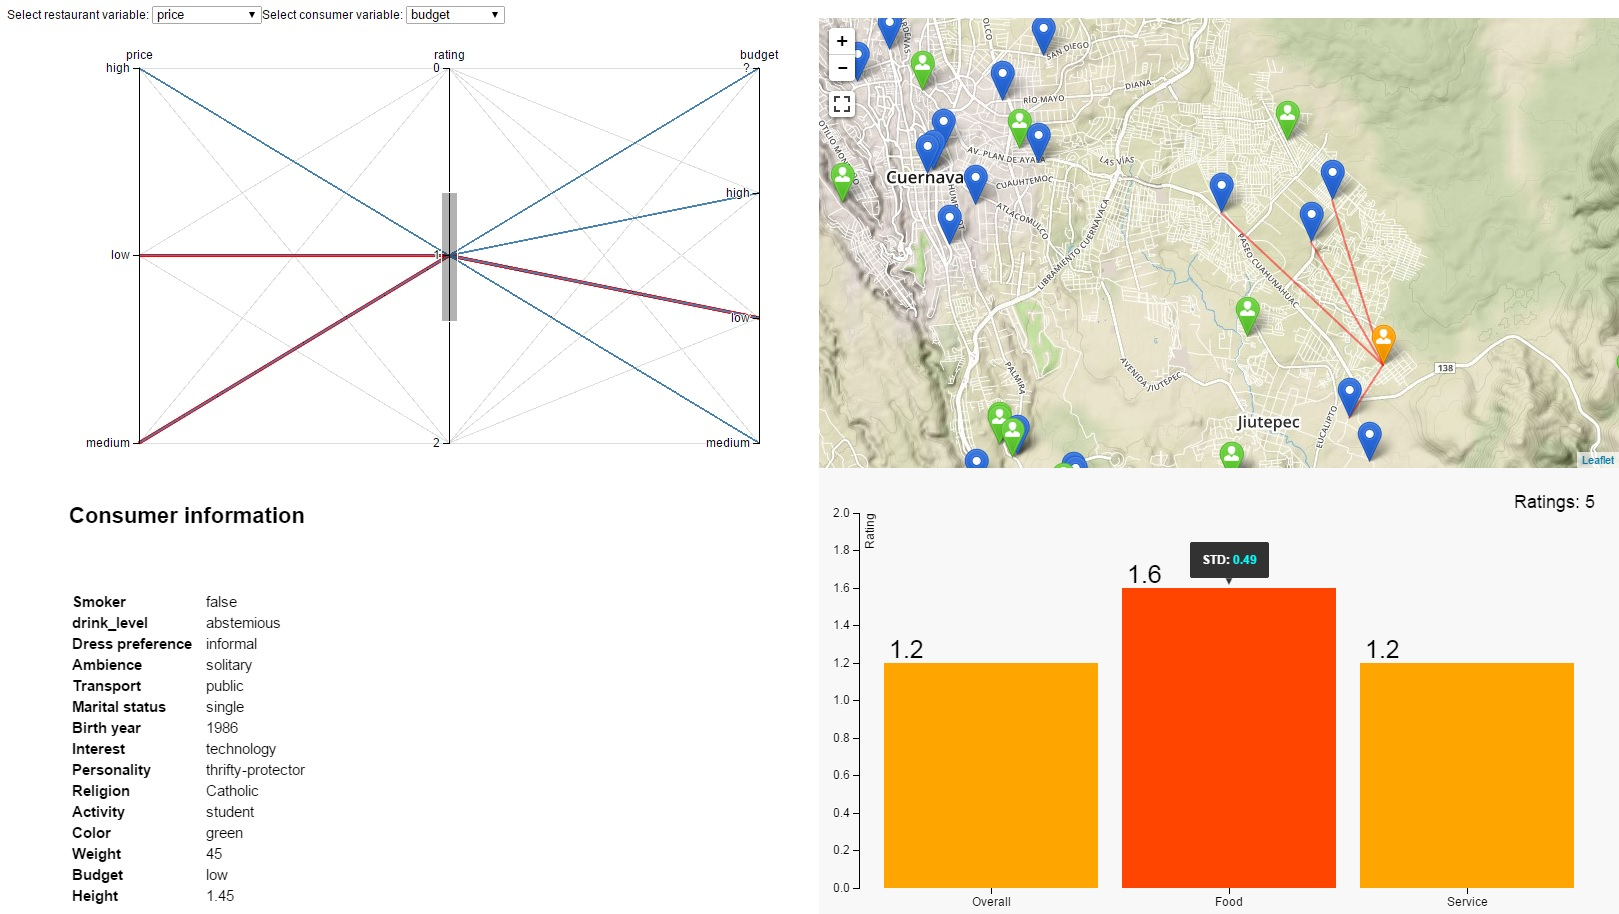
\includegraphics[width=1\textwidth]{img/dashboard-final.jpg}
 \caption{Impression of the multiview dashboard visualization, showing in the left top corner the Parallel Coordinate Plot where a filter has been placed on part of the middle axis}; the geographic map in the top right corner where a consumer marker has been selected; the bar chart in the bottom right corner, indicating the average ratings, as well as the total number of ratings that the selected consumer gave to restaurants; and finally the additional information (user profile attribute values) of the selected user.
 \label{dashboard-view}
\end{figure}

When a consumer or restaurant is selected on the map, more information becomes available in the two bottom views. The view on the left shows additional textual information about the selected consumer or restaurant. The view on the right shows a bar chart, consisting of three bars. Each bar contains the average rating of the selected consumer or restaurant. The left bar shows the average overall rating, the middle shows the average food rating and the last bar shows the average service rating. When the mouse is hovered over one of the bars, the standard deviation of that average rating is shown. The standard deviation can indicate whether or not the ratings given to a restaurant or by a consumer fluctuate a lot.





